\documentclass[../main.tex]{subfiles}

\begin{document}

Reqour deployment is done through CI/CD\footnote{Where \textit{D} stands for deployment, not delivery. Hence, the pipeline is fully automatized.} pipeline. The pipeline consists of 2 main parts: Jenkins (during which \textit{reqour} and \textit{reqour-adjuster} \textbf{JARs} are built and published) and GitLab (during which \textit{reqour} and \textit{reqour-adjuster} \textbf{images} are built and published, as well as deployment being done).

All PNC deployment configs are managed as a part of the internal RedHat GitLab instance, hence, not being publicly available. Because of that, only word descriptions together with diagrams will be present in this chapter.

\section{Jenkins}
\subfile{./sections/jenkins}

\section{GitLab}
\subfile{./sections/gitlab}

Both Jenkins and GitLab parts are visualized (in less detail) in Figure \ref{fig:pipeline}.

\begin{figure}
  \begin{center}
    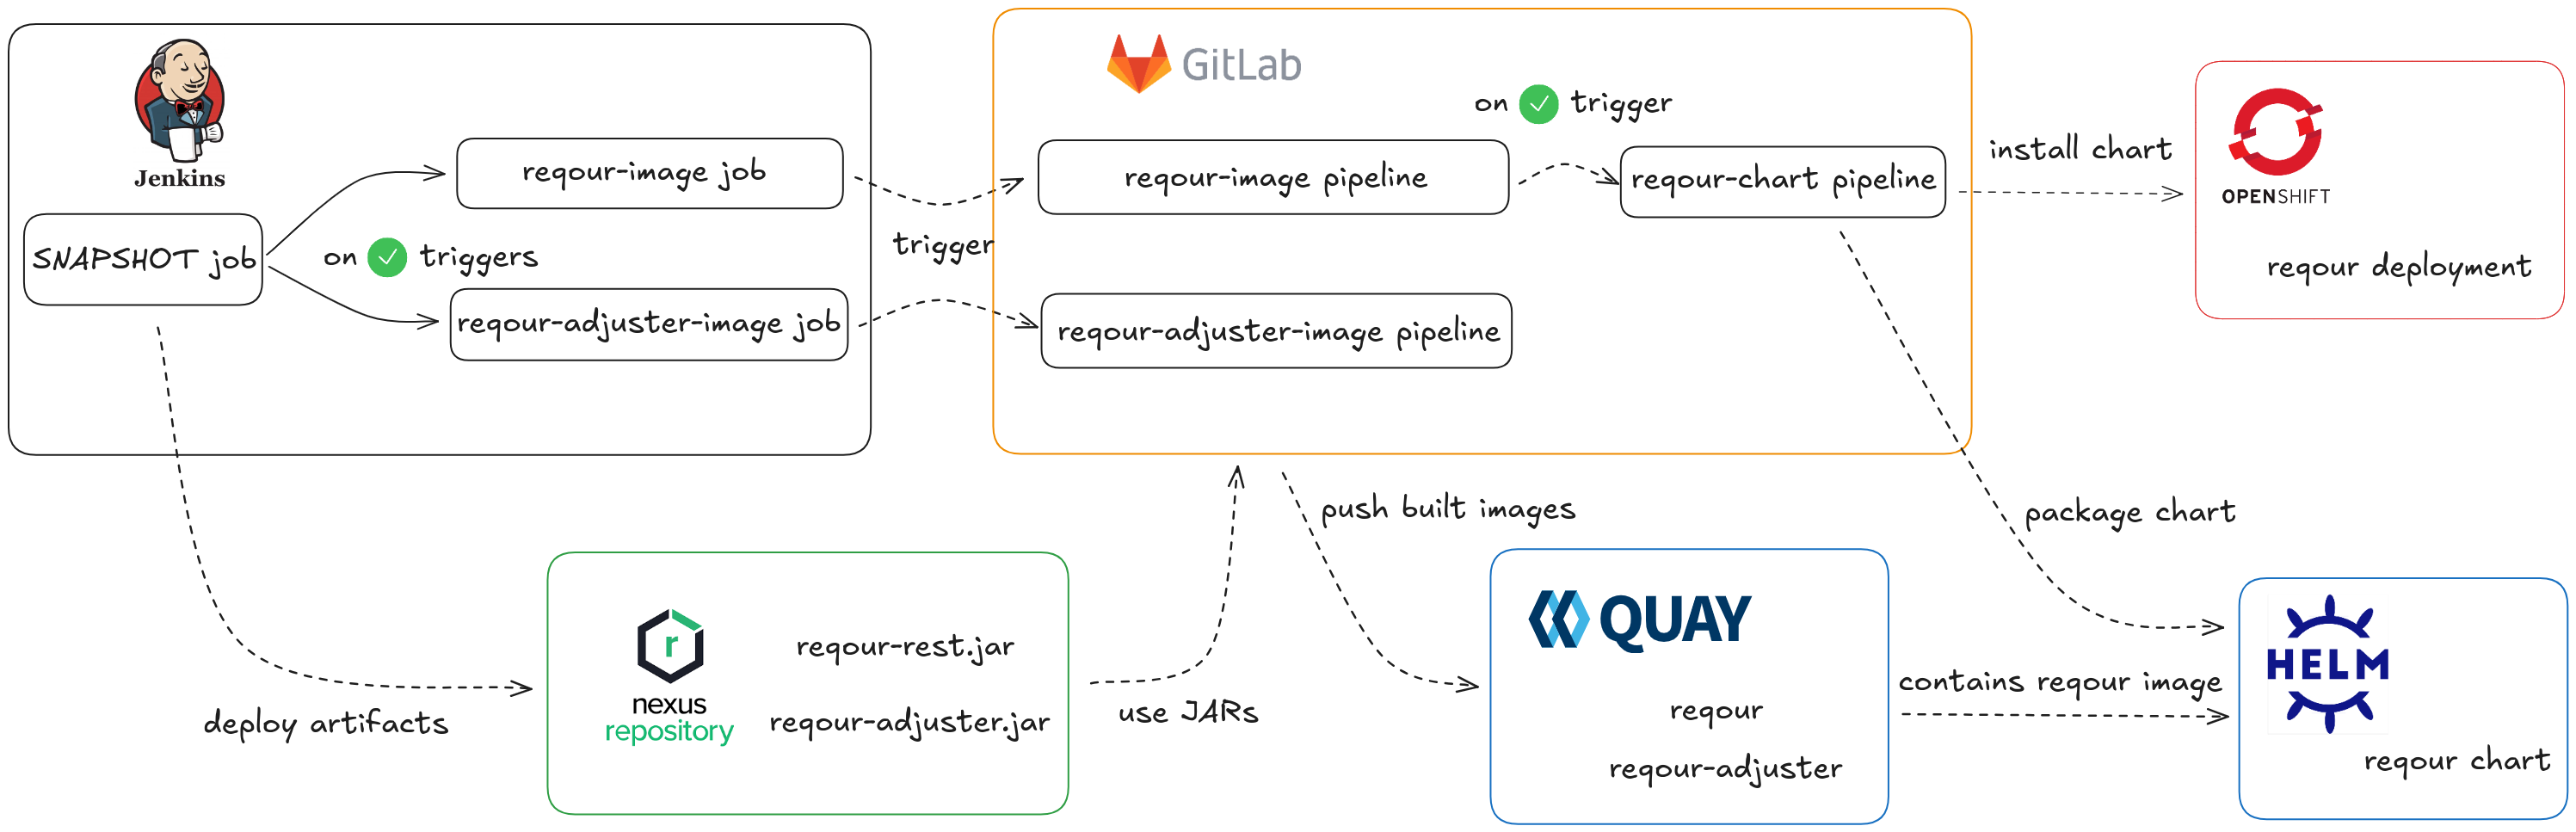
\includegraphics[width=\textwidth]{images/pipeline.png}
  \end{center}
  \caption{Pipeline}
  \label{fig:pipeline}
\end{figure}

\end{document}
